\documentclass[12pt, twoside]{article}
\usepackage[letterpaper, margin=1in, headsep=0.2in]{geometry}
\setlength{\headheight}{0.6in}
%\usepackage[english]{babel}
\usepackage[utf8]{inputenc}
\usepackage{microtype}
\usepackage{amsmath}
\usepackage{amssymb}
%\usepackage{amsfonts}
\usepackage{siunitx} %units in math. eg 20\milli\meter
\usepackage{yhmath} % for arcs, overparenth command
\usepackage{tikz} %graphics
\usetikzlibrary{quotes, angles}
\usepackage{graphicx} %consider setting \graphicspath{{images/}}
\usepackage{parskip} %no paragraph indent
\usepackage{enumitem}
\usepackage{multicol}
\usepackage{venndiagram}

\usepackage{fancyhdr}
\pagestyle{fancy}
\fancyhf{}
\renewcommand{\headrulewidth}{0pt} % disable the underline of the header
\raggedbottom
\hfuzz=2mm %suppresses overfull box warnings

\usepackage{hyperref}

\fancyhead[LE]{\thepage}
\fancyhead[RO]{\thepage \\ Name: \hspace{4cm} \,\\}
\fancyhead[LO]{BECA / Dr. Huson / Geometry\\*  Unit 3: Parallel lines and transversals\\* 17 October 2022}

\begin{document}

\subsubsection*{3.1 Parallel lines and transversals}
\begin{enumerate}
\item Given two parallel lines and a transversal, as shown, with m$\angle 6 =  70^\circ$. Write down the value of each angle measure.
  \begin{multicols}{3}
    \begin{enumerate}[itemsep=0.5cm]
      \item m$\angle 1 = $
      \item m$\angle 2 = $
      \item m$\angle 3 = $
      \item m$\angle 4 = $
      \item m$\angle 5 = $
      \item m$\angle 6 = $
      \item m$\angle 7 = $
      \item m$\angle 8 = $
    \end{enumerate}
      \begin{tikzpicture}[scale=1]
      \draw [<->, thick] (3.5,2)--(7,2);
      \draw [<->, thick] (2.5,0)--(6,0);
      \draw [<->, thick] (4,-1)--(5.5,3);
      \node at (4.5,0.3) [left]{$5$};
      \node at (4.5,0.3) [right]{$6$};
      \node at (4.3,-0.3) [left]{$7$};
      \node at (4.3,-0.3) [right]{$8$};
      \node at (5.2,2) [above left]{$1$};
      \node at (5.2,2) [above right]{$2$};
      \node at (5,2) [below left]{$3$};
      \node at (5,2) [below right]{$4$};
    \end{tikzpicture}
  \end{multicols}

\item Label the relationship of each pair: adjacent, vertical, corresponding, alternate interior, same side interior, alternate exterior, or same side exterior
  \begin{multicols}{2}
    \begin{enumerate}[itemsep=0.5cm]
      \item $\angle 1$,$\angle 4$
      \item $\angle 3$,$\angle 6$
      \item $\angle 5$,$\angle 3$
      \item $\angle 6$,$\angle 2$
      \item $\angle 1$,$\angle 8$
    \end{enumerate}
      \begin{tikzpicture}[scale=1]
      \draw [<->, thick] (3.5,2)--(7,2);
      \draw [<->, thick] (2.5,0)--(6,0);
      \draw [<->, thick] (4,-1)--(5.5,3);
      \node at (4.5,0.3) [left]{$5$};
      \node at (4.5,0.3) [right]{$6$};
      \node at (4.3,-0.3) [left]{$7$};
      \node at (4.3,-0.3) [right]{$8$};
      \node at (5.2,2) [above left]{$1$};
      \node at (5.2,2) [above right]{$2$};
      \node at (5,2) [below left]{$3$};
      \node at (5,2) [below right]{$4$};
    \end{tikzpicture}
  \end{multicols}

\item Identify each angle
  \begin{multicols}{2}
  \begin{enumerate}
    \item Opposite $\angle 4$
    \item Corresponding to $\angle 3$
    \item Alternate exterior to $\angle 8$
    \item Same side interior to $\angle 5$
    \item Alternate interior to $\angle 4$
  \end{enumerate}
  \begin{center}
  \begin{tikzpicture}[scale=1.2]
    \draw [<->, thick] (3,2)--(7,2);
    \draw [<->, thick] (2,0)--(6,0);
    \draw [<->, thick] (4,-1)--(5.5,3);
    \node at (4.5,0.3) [left]{$5$};
    \node at (4.5,0.3) [right]{$6$};
    \node at (4.3,-0.3) [left]{$7$};
    \node at (4.3,-0.3) [right]{$8$};
    \node at (5.2,2) [above left]{$1$};
    \node at (5.2,2) [above right]{$2$};
    \node at (5,2) [below left]{$3$};
    \node at (5,2) [below right]{$4$};
  \end{tikzpicture}
  \end{center}
  \end{multicols} \vspace{2cm}

\newpage
\item Given two parallel lines and a transversal, as shown, with m$\angle 1 =  125^\circ$. Write down the value of each angle measure.
  \begin{multicols}{2}
    \begin{enumerate}[itemsep=0.5cm]
      \item m$\angle 5 = $
      \item m$\angle 6 = $
      \item m$\angle 4 = 5y$. Find $y$.
    \end{enumerate}
      \begin{tikzpicture}[scale=1]
      \draw [<->, thick] (3.5,2)--(7,2);
      \draw [<->, thick] (2.5,0)--(6,0);
      \draw [<->, thick] (4,-1)--(5.5,3);
      \node at (4.5,0.3) [left]{$5$};
      \node at (4.5,0.3) [right]{$6$};
      \node at (4.3,-0.3) [left]{$7$};
      \node at (4.3,-0.3) [right]{$8$};
      \node at (5.2,2) [above left]{$1$};
      \node at (5.2,2) [above right]{$2$};
      \node at (5,2) [below left]{$3$};
      \node at (5,2) [below right]{$4$};
    \end{tikzpicture}
  \end{multicols} \vspace{1.5cm}

\item Given two parallel lines and a transversal, as shown, with m$\angle 6 =  68^\circ$. Write down the value of each angle measure.
  \begin{multicols}{2}
    \begin{enumerate}[itemsep=0.5cm]
      \item What angle is corresponding to $\angle 6$?
      \item What angle is alternate interior to $\angle 4$?
      \item Find m$\angle 1$
    \end{enumerate}
    \begin{flushright}
      \begin{tikzpicture}[scale=1,rotate=20]
      \draw [<->, thick] (3.5,2)--(7,2);
      \draw [<->, thick] (2.5,0)--(6,0);
      \draw [<->, thick] (4,-1)--(5.5,3);
      \node at (4.5,0.3) [left]{$5$};
      \node at (4.5,0.3) [right]{$6$};
      \node at (4.3,-0.3) [left]{$7$};
      \node at (4.3,-0.3) [right]{$8$};
      \node at (5.2,2) [above left]{$1$};
      \node at (5.2,2) [above right]{$2$};
      \node at (5,2) [below left]{$3$};
      \node at (5,2) [below right]{$4$};
    \end{tikzpicture}
  \end{flushright}
  \end{multicols} \vspace{1cm}

\item Given $\triangle ABC$. $\overline{AC} \cong \overline{BC}$,  m$\angle A=48$. Find m$\angle C$.\\[0.5cm]
  \begin{tikzpicture}[scale=0.7]
    \draw[thick](0,0)--(4,0)--(2,6)--(0,0);
    \draw[fill] (0,0) circle [radius=0.05] node[below]{$A$};
    \draw[fill] (4,0) circle [radius=0.05] node[below]{$B$};
    \draw[fill] (2,6) circle [radius=0.05] node[above right]{$C$};
    \draw[thick] (0.8,3.1)--(1.2,2.9); %tick mark
    \draw[thick] (2.8,2.9)--(3.2,3.1);
  \end{tikzpicture}%\vspace{1cm}

\end{enumerate}
\end{document}